\subsection{EMG-forstærker}

EMG-forstærkeren testes for at vurdere, hvorvidt der kan opsamles muskelaktivitet fra rectus femoris. Overfladeelektroderne placeres ud fra SENIAM's anvisning om elektrodeplacering, jf. \autoref{sec:pilotforsoeg}. En squat-øvelse udføres, mens muskelsignaler opsamles i MATLAB. Denne øvelse er beskrevet i \autoref{sec:knaeled_squat}. Muskelsignalet under udførslen af squat-øvelsen fremgår af \autoref{fig:raat_emg}. 

\begin{figure}[H]
\centering
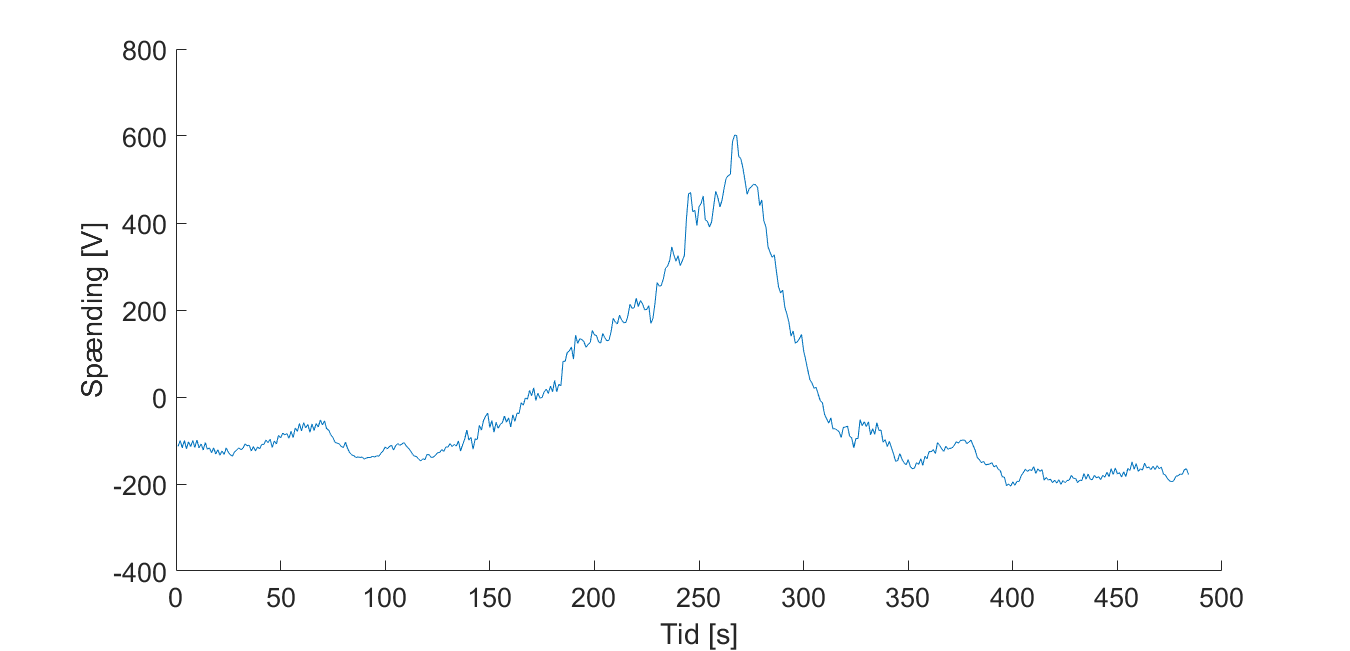
\includegraphics[width=1\textwidth]{figures/raat_EMG_test}
\caption{Et samplede EMG-signal fra rectus femoris under udførsel af en squat-øvelse.}
\label{fig:raat_emg}
\end{figure}

\noindent
Ud fra \autoref{fig:raat_emg} ses det at der opsamles muskelaktivitet fra rectus femoris. For således at undersøge, hvorvidt muskelsignalerne ligger i frekvensområdet mellem $10-500~Hz$ er en frekvensanalyse foretaget. Denne ses af \autoref{fig:fft_raat_emg}

\begin{figure}[H]
\centering
\includegraphics[width=1\textwidth]{figures/fft_raat_EMG}
\caption{Frekvensanalyse af samplet EMG-signal under en squat-øvelse, hvor Y-aksen er en semilogaritmisk skala}
\label{fig:fft_raat_emg}
\end{figure}

\noindent
Det fremgår af \autoref{fig:fft_raat_emg} at signalet ligger inden for frekvensområdet. 
EMG-forstærkerne forsynes med en spænding på $\pm 5,4~V$, hvilket er testet i \autoref{test_spaendingsforsyning}.
På EMG-forstærkeren findes et justerbart gain, således forstærkningen kan tilpasses den enkelte bruger af systemet. Ud fra dette og \autoref{fig:raat_emg} vurderes det, at EMG-forstærkeren opfylder de opstillede krav i \autoref{sec:EMG_krav}.

\vspace{3mm}
\textbf{Opsummering af krav:}
\begin{itemize}
\item[\text{\sffamily \checkmark}] Skal opsamle signaler fra rectus femoris
\item[\text{\sffamily \checkmark}] Skal være anvendeligt med overflade elektroder
\item[\text{\sffamily \checkmark}] Skal opsamle muskelsignaler i frekvensområdet mellem $10-500~Hz$
\item[\text{\sffamily \checkmark}] Skal forsynes med en spænding på minimum $\pm5~V$
\item[\text{\sffamily \checkmark}] Skal have et justerbart gain, der ikke kan forstærke over ADC'ens arbejdsområde
\end{itemize}


\subsection{Accelerometre}

Accelerometrene testes for at vurdere, hvorvidt de opstillede krav i \autoref{sec:acc_teori} opfyldes. 
Det fremgår af databladet, at accelerometrene er triaksiale, samt at accelerometrene kan forsynes med en DC-forsyning fra $1,8-3,6~V$. Kravet hertil er, at accelerometrene skal forsynes med en minimum spænding på $3~V$. Det er derfor testet, hvorvidt om mikrokontrolleren forsyner accelerometrene med denne spænding. Testen er udført ved brug af et multimeter, hvortil der måles en spænding på $3,2~V$. Kravet om den minimum spænding på $3~V$ er derfor opfyldt.
Ud fra målinger foretaget i \autoref{sec:test_acc} ses en linearitet på $0,03~\%$, hvilket derfor lever op til kravet for linearitet. Da det ikke er muligt at teste om accelerometrene har accelerationer i $\pm2~g$, tages der udgangspunkt i databladet. I databladet beskrive det, at accelerometrene har et lineært arbejdsområde på $\pm 3~g$.

\vspace{3mm}
\textbf{Opsummering af krav:}
\begin{itemize}
\item[\text{\sffamily \checkmark}] Skal måle på minimum Y-aksen
\item[\text{\sffamily \checkmark}] Skal forsynes med en spænding på minimum $3~V$
\item[\text{\sffamily \checkmark}] Skal have en linearitet med en afvigelse på $1\%$
\item[\text{\sffamily \checkmark}] Skal måle accelerationer i $\pm2~g$
\end{itemize}

